\documentclass[12pt]{article}  
%%Read the manual for other options. 

\pagestyle{empty} %%Eliminates page numbers
%%\input rmb_macros
%%Collect your favorite macros in a 
%%separate file

%\input amssym.def
%\input amssym
%\input mssymb
%%Defines additional symbols



\usepackage{graphics}
\usepackage{amsmath,amssymb,amsthm, multicol}
\usepackage[pdftex]{graphicx}
\usepackage{epsf}
%%Use to include pictures. 

%\newcommand{\comment}[1]{}
%\newcommand{\sobolev}[2]{W^{#1,#2}}
%\newcommand{\sobolev}[2]{L^#2_#1}
%%Some examples of macros or new commands.

\addtolength{\oddsidemargin}{-.75in}
\addtolength{\evensidemargin}{-.75in}
\addtolength{\textwidth}{1.5in}
\addtolength{\topmargin}{-1in}
\addtolength{\textheight}{2.25in}
%%Set margins, defaults are ok. 

\begin{document}
\begin{center}
{\bf \Large MATH 2B - Integrals and the Fundamental Theorem}
\vspace{0.2cm}
\hrule
\end{center}

\begin{multicols*}{2}
	\begin{enumerate}
		\item If $\int_0^{10}f(x)\ dx = 17$, and $\int_0^8 f(x)\ dx = 12$, find the value of $\int_8^12f(x)\ dx$.
		\vfill
		\item Estimate $\int_0^2 e^{-x^2}\ dx$ using upper and lower bounds.
		\vfill
		\item Evaluate the integral using right endpoints and the definition of the integral.
		\[
		\int_2^5 (4-2x)\ dx
		\]
		\vfill
		\item Interpret the limit as a definite integral over the given interval. Do not evaluate.
		\[
		\lim_{n\to \infty} \sum_{i=1}^n x_i\sqrt{1+x_i^3}\ \Delta x,\quad [2,5]
		\]
		\vfill
		\null
		\columnbreak
		\item Use the graph of $g(x)$ below to evaluate the following integrals by interpreting it in terms of areas. Note that $g$ is composed of two linear functions and a semi-circle.
		\centerline{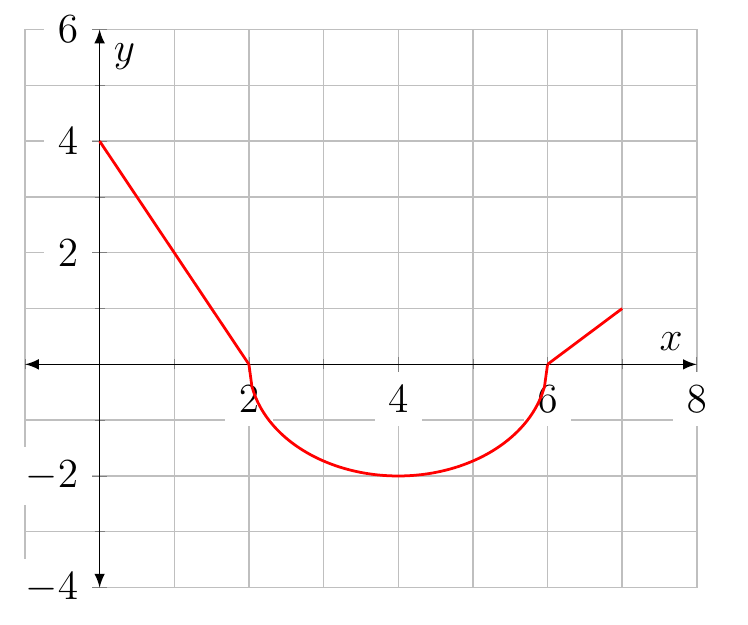
\includegraphics[scale=.4]{graph.png}}
		\begin{enumerate}
			\item \[
			\int_0^2 g(x)\ dx
			\]
			\vfill
			\item \[
			\int_2^6 g(x)\ dx
			\]
			\vfill
			\item \[
			\int_0^7 g(x)\ dx
			\]
			\vfill\null
		\end{enumerate}
		\pagebreak

		\item Use the Fundamental Theorem of Calculus to find the derivative of the function.
		\begin{enumerate}
			\item \[
			g(x) = \int_2^x\ln(1+t^2)\ dt
			\]

			\item \[
			R(y) = \int_y^2 t^3\sin t\ dt
			\]

			\item \[
			h(x) = \int_1^{\sqrt{x}}\frac{z^2}{z^4+1}dz
			\]

			\item \[
			y = \int_0^{x^4}\cos^2\theta\ d\theta
			\]

			\item \[
			y = \int_{\sin x}^1 \sqrt{1+t^2}\ dt
			\]
		\end{enumerate}


		\item Evaluate the integral.
		\begin{enumerate}
			\item \[
			\int_{-5}^5 e\ dx
			\]

			\item \[
			\int_0^1\cosh t\ dt
			\]

			\item \[
			\int_1^{18}\sqrt{\frac{3}{z}}\ dz
			\]

			\item \[
			\int_{1/2}^{1/\sqrt{2}}\frac{4}{\sqrt{1-x^2}}dx
			\]
		\end{enumerate}

		\item Find $\int_{-2}^2 f(x)\ dx$ where 
		\[
		f(x) = \begin{cases}
			2& \text{if }-2\leq x\leq 0\\
			4-x^2 & \text{if }0<x\leq 2
		\end{cases}.
		\]

		\columnbreak

		\item Find the derivative of the function.
		\begin{enumerate}
			\item \[
			F(x) = \int_x^{x^2}e^{t^2}dt
			\]

			\item \[
			y = \int_{\cos x}^{\sin x}\ln(1+2v)\ dv
			\]
		\end{enumerate}

		\vfill

		\item Let $g(x) = \int_0^x f(t)dt$, where $f$ is the function whose graph is shown.
		\begin{enumerate}
			\item At what values of $x$ do the local maximum and minimum values of $g$ occur?
			\item Where does $g$ attain its absolute maximum value?
			\item On which intervals is $g$ concave downward?
		\end{enumerate}
		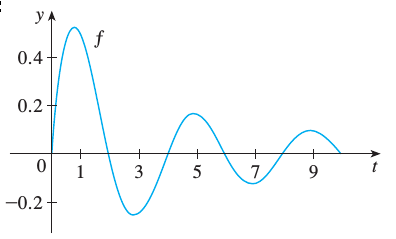
\includegraphics[scale=.6]{74_pic.png}

		\vfill

		\item Show that this expression does not depend on $x$. (That is, show that its derivative with respect to $x$ is zero).
		\[
		\int_0^x \frac{dt}{1+t^2} + \int_0^{1/x}\frac{dt}{1+t^2}.
		\]

		\vfill\null\pagebreak
	\end{enumerate}
\end{multicols*}


h
\end{document}